
\documentclass[a4paper,10pt,parskip=half]{scrbook}

\usepackage[usenames,dvipsnames]{xcolor}
\usepackage{graphicx}
\usepackage[utf8]{inputenc} %-- pour utiliser des accents en français
\usepackage{mathpazo}
\usepackage{amsmath,amssymb,amsthm} 
\usepackage[square]{natbib}
\usepackage{url}
\usepackage{xspace}
\usepackage[left=25mm,top=25mm]{geometry}
% \usepackage{geometry}
\usepackage[ruled,vlined,linesnumbered]{algorithm2e}
\usepackage{subcaption}
\usepackage{booktabs}
\usepackage{listings}
\usepackage{cancel}
\usepackage{colortbl}
\usepackage{lastpage}
\usepackage{todonotes}
\usepackage{fontawesome}
\usepackage{ccicons}
\usepackage{textcomp}
\usepackage{gensymb}
\usepackage{float}
\usepackage{tikz}
\usepackage[tikz]{mdframed}
\usepackage[UKenglish]{isodate}% http://ctan.org/pkg/isodate

\definecolor{colourforlinks}{rgb}{0.28, 0.5, 0.5}
\usepackage[unicode=true,
            breaklinks=true,
            colorlinks=true,
            allcolors=colourforlinks,
            % pagebackref=true,
            linktoc=page,
            pdftitle={Computational modelling of terrains},
            pdfauthor={Hugo Ledoux, Ken Arroyo Ohori, Ravi Peters}]{hyperref}


\usepackage{bibentry}
\nobibliography*

\newcommand{\ie}{ie}
\newcommand{\eg}{eg}
\newcommand{\reffig}[1]{Figure~\ref{#1}}
\newcommand{\refsec}[1]{Section~\ref{#1}}
\newcommand{\refchap}[1]{Chapter~\ref{#1}}


\setcapindent{1em} %-- for captions of Figures
\setcounter{tocdepth}{\sectiontocdepth}
% \setcounter{tocdepth}{\subsectiontocdepth}


% \renewcommand{\refname}{References \& further reading}
\renewcommand{\contentsname}{\vspace{-15mm}}

\definecolor{light-gray}{gray}{0.97}
\definecolor{myred}{RGB}{111,12,31}
\definecolor{mygreen}{RGB}{35,138,35}

\newfloat{myfloat}{thp}{lop}

\newmdenv[%
  outerlinewidth=1.5,%
  roundcorner=5pt,%
  linecolor=myred,%
  backgroundcolor=light-gray,%
  frametitle=\faExternalLink\ To read or watch,
]{link-box}

\newmdenv[%
  outerlinewidth=1.5,%
  roundcorner=5pt,%
  linecolor=mygreen,%
  backgroundcolor=light-gray,%
  frametitle=\faCog\ How does it work in practice?,
]{practice-box}


\title{Post-primary School Mathematics}
\author{Ronan Downes}
\date{v0.1.1}




\publishers{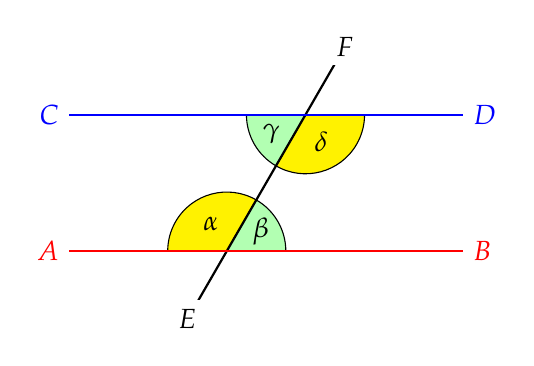
\begin{tikzpicture}
\draw[fill=yellow] (0,0) -- (60:.75cm) arc (60:180:.75cm);
\draw(120:0.4cm) node {$\alpha$};
\draw[fill=green!30] (0,0) -- (right:.75cm) arc (0:60:.75cm);
\draw(30:0.5cm) node {$\beta$};
\begin{scope}[shift={(60:2cm)}]
\draw[fill=green!30] (0,0) -- (180:.75cm) arc (180:240:.75cm);
\draw (30:-0.5cm) node {$\gamma$};
\draw[fill=yellow] (0,0) -- (240:.75cm) arc (240:360:.75cm);
\draw (-60:0.4cm) node {$\delta$};
\end{scope}
\begin{scope}[thick]
\draw (60:-1cm) node[fill=white] {$E$} -- (60:3cm) node[fill=white] {$F$};
\draw[red] (-2,0) node[left] {$A$} -- (3,0) node[right]{$B$};
\draw[blue,shift={(60:2cm)}] (-3,0) node[left] {$C$} -- (2,0) node[right]{$D$};
\draw[shift={(60:1cm)},xshift=4cm];
% node [right,text width=6cm,rounded corners,fill=red!20,inner sep=1ex]
% {
% When we assume that $\color{red}AB$ and $\color{blue}CD$ are
% parallel, i.\,e., ${\color{red}AB} \mathbin{\|} \color{blue}CD$,
% then $\alpha = \delta$ and $\beta = \gamma$.
% };
\end{scope}
\end{tikzpicture}}




% \publishers{\begin{tikzpicture}
% \draw[fill=yellow] (0,0) -- (60:.75cm) arc (60:180:.75cm);
% \draw(120:0.4cm) node {$\alpha$};
% \draw[fill=green!30] (0,0) -- (right:.75cm) arc (0:60:.75cm);
% \draw(30:0.5cm) node {$\beta$};
% \begin{scope}[shift={(60:2cm)}]
% \draw[fill=green!30] (0,0) -- (180:.75cm) arc (180:240:.75cm);
% \draw (30:-0.5cm) node {$\gamma$};
% \draw[fill=yellow] (0,0) -- (240:.75cm) arc (240:360:.75cm);
% \draw (-60:0.4cm) node {$\delta$};
% \end{scope}
% \begin{scope}[thick]
% \draw (60:-1cm) node[fill=white] {$E$} -- (60:3cm) node[fill=white] {$F$};
% \draw[red] (-2,0) node[left] {$A$} -- (3,0) node[right]{$B$};
% \draw[blue,shift={(60:2cm)}] (-3,0) node[left] {$C$} -- (2,0) node[right]{$D$};
% \draw[shift={(60:1cm)},xshift=4cm];
% % node [right,text width=6cm,rounded corners,fill=red!20,inner sep=1ex]
% % {
% % When we assume that $\color{red}AB$ and $\color{blue}CD$ are
% % parallel, i.\,e., ${\color{red}AB} \mathbin{\|} \color{blue}CD$,
% % then $\alpha = \delta$ and $\beta = \gamma$.
% % };
% \end{scope}
% \end{tikzpicture}}







% \publishers{\includegraphics[width=\linewidth]{front-back/quebec.jpg}}

%-- remove the 'rd' in '23rd June' --> '23 June'


\usepackage{pst-coil,pstricks-add}
\usepackage[nomessages]{fp}

\FPset\CoilArm{0.25}
\FPset\CoilWidth{0.3}
\FPeval\CoilTurn{round(50/3:3)}
\FPeval\DeltaY{0.5}
\FPeval\Amp{1.5}
\FPeval\FPS{25}
\FPeval\Vx{2}% propagation speed
\FPeval\Period{1}% second

\psset
{
    coilarm=\CoilArm,
    coilwidth=\CoilWidth,
}


\newcommand\System[4][0]{% #1: frame, #2: x, #3: y, #4: label
    \uput[90](#2,4.25){#4}
    \FPeval\CoilHeight{round((4-(#3)-2*CoilArm)/(CoilWidth*CoilTurn):3)}
    \pszigzag[coilheight=\CoilHeight,linejoin=2](#2,4)(#2,#3)
    \ifnum#1=1
        \bgroup
            \psset{origin={#2,#3}}
            \psframe[dimen=inner,fillstyle=solid,fillcolor=black](-0.5,0)(0.5,-1)
            \psdot[linecolor=yellow](0,-0.5)
        \egroup
    \fi
}


\cleanlookdateon

\begin{document}

%-------------------------------------------
\frontmatter
\maketitle

\clearpage
\include{front-back/pre}
\include{front-back/preface}

\tableofcontents
% \listoffigures
% \listoftables


%-------------------------------------------
\mainmatter
\include{NUM/number00-part}

\label{chap:numbersystems}




\chapter{\protect\hyperlink{chap:\thechapter}{Numeral and Number systems}}
\addtocontents{toc}{\protect\hypertarget{chap:\thechapter}{}}
\LARGE

\section{Integers and decimals}
Maths is divided in two based on whether the quantities involved have gaps or not. It there are gaps then we can use counting to  describe the  "how much?" or "how many?" questions and our answer is always an integer.  If there are no gaps then we can measure the quantity to any level of precision and we use decimals for that.  Some situations can only give positive integer answers or non-negative answers but these \textbf{Natural Numbers} and \textbf{Whole Numbers} are just a type of integer and it is important that you appreciate that the most important distinction in maths between our number systems is that some are \textbf{discrete} and use integers and other are continuous and use  decimals. 

Remember the gaps mean integers, no gaps means decimals. That is the big powerful idea you need to remember.
\section{Fractions, decimals, percentages  }












\section{Counting Is Arithmetic}
You have probably already learned  how to count! You may be saying: “But I already know how to count: one, two, three, $\ldots$”

True. But most counting problems do not involve simply counting a list or group of items. Usually we have to first figure out what we’re counting, then we have to figure out how to count it.

One thing that we will repeat over and over in this chapter, and indeed in the course of the entire book, is:

\begin{claim}
Don’t memorize!
\end{claim}



\section{Defining thereoms}
Theorems can easily be defined
\newtheorem{prop}{Proposition}[section]
\begin{theorem}
Let $f$ be a function whose derivative exists in every point, then $f$ is 
a continuous function.
\end{theorem}

\begin{theorem}[Pythagorean theorem]
\label{pythagorean}
This is a theorema about right triangles and can be summarised in the next 
equation 
\[ x^2 + y^2 = z^2 \]
\end{theorem}

And a consequence of theorem \ref{pythagorean} is the statement in the next 
corollary.

\begin{corollary}
There's no right rectangle whose sides measure 3cm, 4cm, and 6cm.
\end{corollary}

You can reference theorems such as \ref{pythagorean} when a label is assigned.

\begin{lemma}
Given two line segments whose lengths are $a$ and $b$ respectively there is a 
real number $r$ such that $b=ra$.
\end{lemma}

\section{}




\section{}

\section{}



\section{}


\section{}







\section{}




\section{}








\section{}
% \includegraphics[width=20mm]{Images/sm-001.jpg}

\chapter{\protect\hyperlink{chap:\thechapter}{Properties of Arithmetic}}
\addtocontents{toc}{\protect\hypertarget{chap:\thechapter}{}}



\section{Why Start with Arithmetic?}
Arithmetic refers to the basics of adding, subtracting, multiplying, dividing, and (maybe) more exotic things like squares and square roots.
But you already know how to add, subtract, multiply, and divide  so why do we have an entire chapter on the properties arithmetic?  You probably learned most of these basics already. The hardest thing that you usually do in arithmetic is “word problems” like “If Jenny has 5 apples and Timmy has 7 apples, then how many apples do they have together?” As you get older, the numbers get bigger, but the problems don’t really get much harder. Arithmetic is great when trying to solve simple problems like counting apples. But when the problems get more complicated we will need Algebra.


\begin{problem}
This is a problem
\end{problem}


\begin{connection}
The properties and vocabulary you focus on here will be used in Algebra and Sets and so are not confined to use with arithmetic. The Number Strand prepares us for and leads on to the Algebra Strand and so in post-primary school we study Number with concepts and language that will form a bridge between Number and Algebra. Some books name this bridge \textbf{prealgebra} . What is prealgebra?  Prealgebra is the bridge between arithmetic and algebra.
\end{connection}






 



To take a simple example, you can use arithmetic to show that\[ 2 \times (3 + 5) = (2 \times 3) + (2 \times 5), \]because the left side equals $2 \times 8$, which is 16, and the right side equals $6 + 10$, which is also 16. But algebra gives us the much more general tool that\[ a \times (b + c) = (a \times b) + (a \times c), \]no matter what numbers $a$, $b$, and $c$ are. While this implies that the letters are \textbf{variables} $a$, $b$, and $c$ might even become \textbf{expressions} and    \textbf{sets} and an exotic number called a \textbf{complex numbers} \footnote{These are numbers that you don't have to worry about or recognise until you are in TY and Leaving Certificate maths!} Even more generally, “$+$” and “$\times$” might not mean addition and multiplication as you think of them now, but instead might represent more complicated mathematical operations when we study \textbf{sets}  so rest assured careful thinking and mastering of the vocabulary we use here is very important.

Our initial goal,lay down the rules of arithmetic, and to give you some ideas as to why these rules are true. Once you know the rules, you’ll be ready to start thinking algebraically.

Also, by the time you start reading this book, you are mathematically mature enough to start thinking about not just how to perform various calculations, but why the techniques used in those calculations work. Understanding why mathematics works is the key to solving harder problems. If you only understand how techniques work but not why they work, you’ll have a lot more difficulty modifying those techniques to solve more complicated problems. So, throughout this book, we will rarely just tell you how something works–we’ll usually show you why it works.

By the end of this chapter, you should be able to explain why the following computations are true:

\section{Basic computation}




\section{Commutative Law of Addition}


\begin{figure*}[h!]
   \centering
    \href{https://www.geogebra.org/m/CsDdkudm}{\includegraphics[width=.6\textwidth]{Images/sm-001.jpg}}
    \caption{\href{https://www.geogebra.org/m/CsDdkudm}{Click anywhere to explore the Commutative Law of Addition.}}
\end{figure*}














\section{Commutative Law of Addition}
\begin{figure}%[4]
    \centering
    \href{https://www.geogebra.org/m/CsDdkudm}{\includegraphics[width=.6\textwidth]{Images/sm-000.jpg}}
    \caption{\href{https://www.mathopenref.com/trianglecircumcircle.html}{Click anywhere to explore the circumcentre and circumcircle of a triangle.}}
\end{figure}



\section{perform mixed arithmetic operations of positive
integers involving multiple levels of brackets}












\section{understand the concept of power}




\section{Enrichment Material marked with asterisks$^*$}

\section{HL only material is underlined}



\section{Expanded Media}


\section{Comparing Completion and Reduction}
N.3 investigate situations involving proportionality so that they can:
a. use absolute and relative comparison where appropriate
b. solve problems involving proportionality including those involving currency conversion
and those involving average speed, distance, and time
\include{whatisterrain/whatisterrain} %- 01
\include{acquisition/acquisition} %- 02
% \include{dtvd/dtvd} %- 03
% \include{interpol/interpol} %- 04
% \include{kriging/kriging} %- 05
% \include{topofeatures/topofeatures} %- 06
% \include{runoff/runoff} %- 07
% \include{conversion/conversion} %- 08
% \include{spatialextent/spatialextent} %- 09
% \include{massive/massive} %- 10
% \include{visibility/visibility} %- 11
% \include{pcprocessing/pcprocessing} %- 12
% \include{bathymetry/bathymetry} %- 13


%-------------------------------------------
\backmatter 
\bibliographystyle{refs/tb.bst} 
\bibliography{refs/tb}

\cleardoublepage
\thispagestyle{empty}

\end{document}
